
\documentclass[a4paper,12pt]{article}
\usepackage{cancel}
\usepackage{url}
\usepackage{xcolor}
\usepackage{hyperref}
\usepackage{amsmath,amsthm,amssymb}
\usepackage{mathtext}
\usepackage[T1,T2A]{fontenc}
\usepackage[utf8]{inputenc}
\usepackage[english,russian]{babel}
\usepackage{wrapfig}
\usepackage{graphicx}
\graphicspath{{pictures/}}
\DeclareGraphicsExtensions{.pdf,.png,.jpg}

\usepackage[a4paper,width=150mm,top=20mm,bottom=20mm, left=30mm, right=20mm]{geometry}
\definecolor{linkcolor}{rgb}{0,0,1} % цвет ссылок
\definecolor{urlcolor}{rgb}{0,0,1} % цвет гиперссылок
	
\renewcommand{\theequation}{\thesection.\arabic{equation}}
 
\hypersetup{pdfstartview=FitH,  linkcolor=linkcolor,urlcolor=urlcolor,citecolor=urlcolor, colorlinks=true}
 
 \makeatletter

 \makeatother

\begin{document}


%\vspace{2cm}
%\LARGE
%\vspace{1cm}
\begin{center}
	
	
	\large
    Министерство образования Российской Федерации\\
    \vspace{1cm}
	Федеральное государственное автономное образовательное учреждение
		высшего профессионального образования\\
		"Московский физико-технический институт (национальный исследовательский университет)"\\
	\vspace{0.5cm}
    Физтех-школа фундаментальной и прикладной физики\\
    \vspace{0.5cm}
	Факультет проблем физики и энергетики\\
	\vspace{0.5cm}
	Кафедра электродинамики сложных систем и нанофотоники\\
	\vspace{2cm}
	\textbf{Исследование свойств оптических волокон с брэгговскими решётками для сенсорных применений} \\
	Выпускная квалификационная работа\\
	(бакалаврская работа)\\
	\vspace{1cm}
	Направление подготовки: 03.03.01 Прикладные математика и физика
	%\end{framed}
	
	%\LARGE
\end{center}
\vspace{1.0cm}
Работу выполнил:\\ 
студент 685 группы\hspace{1.7cm}\underline{\hspace{2.8cm}}\hspace{0.5cm}Барсегян Сергей Симонович\\
\vspace{1.0cm}\\
Научный руководитель:\\
д.ф.-м.н.\hspace{2.7cm}\underline{\hspace{2.8cm}}\hspace{0.5cm}Дорофеенко Александр Викторович\\

\begin{center}
	\vspace{5cm}
	{Москва, 2020}
\end{center}

\thispagestyle{empty}

\pagebreak[4]
\setcounter{page}{1} 

%\vspace{\fill}



\tableofcontents{}

\pagebreak[4]


\renewcommand{\theequation}{\arabic{equation}}


\addcontentsline{toc}{section}{Введение}






\section*{Введение}\label{intro}

Индуцирование плазмонного резонанса в системе с напылением проводящего слоя на диэлектрики различной конфигурации (призма или цилиндр ) открывают возможность создать очень чувствительный к внешним параметрам сенсор.

\begin{figure}[h!]
	\centering
	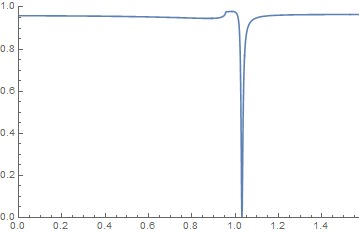
\includegraphics[width=0.5\linewidth]{kretchmann}
	\caption{Эффект Кречмана}\label{fig:kretchmann}
\end{figure}



Физическое явление которое легло в основание данной схемы было предложено Кречманом и Отто. Для производства сенсоров наиболее применимой и удобной является схема Кречмана которая является фундаментом для построения схемы расмотренной в данной работе.
Световой пучок падает на ~\ref{fig:sandwitch} сэндвич из диэлектрика с $ \varepsilon_p >1 $ и слоя с металлическим напылением испытывая полное внутренне отражаение. В идеалированной ситуации коэффицент отражения равен единице, однако при некотором угле падение возникает резкое падение ~\ref{fig:kretchmann}коэффицента отражения вызванное скачком интенсивности поля у металла. В литературе это называют нарушенным полным внутренним отражением (НПВО).

Данная конфигурация очень полезна так-как позволяет посчитать $ \varepsilon $ среды граничащей с металлом по расположению скачка коэффицента отражения из-за чувствительности данной схемы к свойствам материала.

В данной же работе будет исследована цилиндрическая конфигурация с наклонной брегговской решёткой.


\begin{center}
	\begin{figure}[h]
		\centering
		\begin{tikzpicture}
		
		\node[] at (60:1.5)  {$\theta$};
		\node[] at (35:1)  {$\alpha$};
		\node[] at (12:6.2)  {$\beta$};
		\coordinate (fov) at (2, 1);
		
		\draw[thick,blue, snake=coil,segment aspect=0.15] (fov) -- ++(220:1.5cm);
		\draw[thick,red, snake=coil,segment aspect=0.15] (fov) -- ++(150:3cm);
		\draw[thick,green, snake=coil,segment aspect=0.15] (5,1) -- ++(30:2cm);
		
		\draw[thick] (1,1) arc (180:215:1) ;
		\draw[thick] (0.9,1) arc (180:150:1) ;
		\draw[thick] (5.7,1) arc (0:30:0.6) ;
		\draw[thick,->](8,1) -- (-1,1)  ;
		
		
		\definecolor{color1}{RGB}{252,156,12};
		\definecolor{color2}{RGB}{252,124,12};
		\definecolor{color3}{RGB}{252,104,12};
		\fill[fill=color1,opacity=.7]  (2,0) rectangle (3,2) ;
		\fill[fill=color2,opacity=.7]  (3,0) rectangle (4,2) ;
		\fill[fill=color3,opacity=.7]  (4,0) rectangle (5,2) ;
		\end{tikzpicture}
		\caption{Трёхслойная среда с показателями преломления $ n_1, n_2, n_3 $}\label{fig:sandwitch}
	\end{figure}
	
	
\end{center}






\section{Эффекти Кречмана}
\begin{center}
	\begin{tikzpicture}
	
	\node[] at (60:1.5)  {$\theta$};
	\node[] at (35:1)  {$\alpha$};
	\node[] at (12:6.2)  {$\beta$};
	\coordinate (fov) at (2, 1);
	
	\draw[thick,blue, snake=coil,segment aspect=0.15] (fov) -- ++(220:1.5cm);
	\draw[thick,red, snake=coil,segment aspect=0.15] (fov) -- ++(150:3cm);
	\draw[thick,green, snake=coil,segment aspect=0.15] (5,1) -- ++(30:2cm);
	
	\draw[thick] (1,1) arc (180:215:1) ;
	\draw[thick] (0.9,1) arc (180:150:1) ;
	\draw[thick] (5.7,1) arc (0:30:0.6) ;
	\draw[thick,->](8,1) -- (-1,1)  ;
	
	
	\definecolor{color1}{RGB}{252,156,12};
	\definecolor{color2}{RGB}{252,124,12};
	\definecolor{color3}{RGB}{252,104,12};
	\fill[fill=color1,opacity=.7]  (2,0) rectangle (3,2) ;
	\fill[fill=color2,opacity=.7]  (3,0) rectangle (4,2) ;
	\fill[fill=color3,opacity=.7]  (4,0) rectangle (5,2) ;
	\end{tikzpicture}
\end{center}



Рассмотрим падение света на слоистую среду под углом $ 
\theta_1 $ с коэффицентами  диэлектрическими проницаемостями $ \varepsilon_1, \varepsilon_2, \varepsilon_3 $ соответственно. 
На границе каждой среды можно записать закон Снеллиуса.

	$$
	\frac{\sin{\theta_2}}{\sin{\theta_1}} = \frac{n_2}{n_1} =\sqrt{\frac{\varepsilon_{2}}{\varepsilon_1}}	$$
	$$
	\frac{{\sin\theta_3}}{\sin{\theta_2}} = \frac{n_3}{n_2} =\sqrt{\frac{\varepsilon_{3}}{\varepsilon_2}}	
	$$

Наша цель посчитать коэфиценты отражение и прохождения для такой слоистой системы. В это задаче очень полезен метод $ T $-матриц. Обозначим коэффицент отражения через $ r $ , f коэффицент прохождения через $ t $.

Тогда на матричном языке можно задать взаимосвязь между этими величинами. А именно распишем ампплитуды волн слева и справа.

$$\vec{E}=\vec{E}(x) e^{i(\omega t-\beta z)}$$

$$E(x)=\left\{\begin{array}{c}
E_{1} e^{i k_{1} x}+E_{1}^{\prime} e^{-i k_{1} x}, x<0 \\
E_{2} e^{i k_{2 x} x}+E_{2}^{\prime} e^{-i k_{2} x_{2} x}, 0<x<d \\
E_{3} e^{i k_{3}(x-d)}+E_{3}^{\prime} e^{-i k_{3}(x-d)}, x>d
\end{array}\right.$$

$$P_{2}=\left(\begin{array}{cc}
e^{i k_{2 x} d} & 0 \\
0 & e^{-i k_{2 x} d}
\end{array}\right)$$



$$
S_{21} = 
\frac{1}{2 Z_2}\begin{pmatrix}
	Z_2+Z_1 & Z_2 -Z_1 \\
	Z_2-Z_1 & Z_2+Z_1
\end{pmatrix}
$$


$$
S_{32} = 
\frac{1}{2 Z_3}\begin{pmatrix}
Z_3+Z_2 & Z_3 -Z_2 \\
Z_3-Z_2 & Z_3+Z_2
\end{pmatrix}
$$

Где $Z_i = \frac{k_{zi}}{k_0}$ для $ s $ - поляризации и $Z_i = \frac{k_{zi}}{\varepsilon_i k_0}$ для $ p $ - поляризации 

$$
 k_{zi} = \sqrt{k_0^2 \epsilon_i - k_x^2)}
$$

$$
 k_{x} = k_0 \sin{ \theta}
$$


$
S_{32} P_2 S_{21} \begin{pmatrix}
	1\\
	r 
\end{pmatrix} = 
\begin{pmatrix}
t\\
0 
\end{pmatrix}
$






\section{Моды волновода}

Для расчёта мод в волноводе имеющую форму цилиндра и состоящую из двух слоёв с показателями преломления $ n_1 $ и $ n_2 $ удобно перейти к цилиндрической систем координат. Так-как предполагается что волновод  однороденны вдоль оси цинлиндра зависисмотсь от $ z $ и $ t $ может быть взята в виде $\exp (i h z-i \omega t)$
Запишем Уравнения Максвелла:
$$\operatorname{rot} \mathbf{H}=\frac{\partial D}{\partial t}, \quad \operatorname{rot} \mathbf{E}=-\frac{\partial B}{\partial t}$$

В цилиндрической системе координат они примут вид:

$$\frac{1}{r} \frac{\partial H_{z}}{\partial \varphi}-\frac{\partial H_{\varphi}}{\partial z}=-i \omega \varepsilon E_{r}, \frac{\partial H_{r}}{\partial z}-\frac{\partial H_{z}}{\partial r}=-i \omega \varepsilon E_{\varphi}$$

$$\frac{1}{r} \frac{\partial}{\partial r}\left(r H_{\varphi}\right)-\frac{1}{r} \frac{\partial H_{r}}{\partial \varphi}=-i \omega \varepsilon E_{z}$$

$$\frac{1}{r} \frac{\partial E_{z}}{\partial \varphi}-\frac{\partial E_{\varphi}}{\partial z}=i \omega \mu H_{r}, \quad \frac{\partial E_{r}}{\partial z}-\frac{\partial E_{z}}{\partial r}=i \omega \mu H_{\varphi}$$

$$\frac{1}{r} \frac{\partial E_{z}}{\partial \varphi}-\frac{\partial E_{\varphi}}{\partial z}=i \omega \mu H_{r}, \quad \frac{\partial E_{r}}{\partial z}-\frac{\partial E_{z}}{\partial r}=i \omega \mu H_{\varphi}$$

$$\frac{1}{r} \frac{\partial}{\partial r}\left(r E_{\Phi}\right)-\frac{1}{r} \frac{\partial E_{r}}{\partial \varphi}=i \omega \mu H_{z}$$


Из этих уравнений поперечные компоненты полей $E_{r}, E_{\varphi}, H_{r}, H_{\Phi}$

можно записать через продольные составляющие $E_{z}, H_{z}$

$$E_{r}=\frac{1}{k^{2}-h^{2}}\left(ih \frac{\partial E_{z}}{\partial r}+\frac{i \omega \mu}{r} \frac{\partial H_{s}}{\partial \varphi}\right)$$

$$E_{\varphi}=\frac{1}{k^{2}-h^{2}}\left(\frac{i h}{r} \frac{\partial E_{z}}{\partial \varphi}-i \omega \mu \frac{\partial H_{z}}{\partial r}\right)$$

$$H_{r}=\frac{1}{k^{2}-h^{2}}\left(\text { ih } \frac{\partial H_{\mathbf{z}}}{\partial r}-\frac{i \omega \mathbf{e}}{r} \frac{\partial E_{\mathbf{z}}}{\partial \varphi}\right)$$


$$H_{\varphi}=\frac{1}{k^{2}-h^{2}}\left(\frac{i h}{r} \frac{\partial H_{z}}{\partial \varphi}+i \omega e \frac{\partial E_{z}}{\partial r}\right)$$


Продольные компоненты полей удоволетворяют волновому уравнению

$$\frac{\partial^{2} U}{\partial r^{2}}+\frac{1}{r} \frac{\partial U}{\partial r}+\frac{1}{r^{2}} \frac{\partial^{2} U}{\partial \varphi^{2}}+\left(k^{2}-h^{2}\right) U=0$$


$$U=F(r) e^{t m \varphi}$$


$$u^{2}=k^{2}-h^{2}$$

$$\frac{\partial^{2} F}{\partial r^{2}}+\frac{1}{r} \frac{\partial F}{\partial r}+\left(u^{2}-\frac{m^{2}}{r^{2}}\right) F=0$$


$$E_{z}^{(t)}=\sum_{m=-\infty}^{\infty} A_{m} J_{m}(u r) \cos m \varphi \exp (i h z-i \omega t)$$


$$H_{z}^{(1)}=\sum_{m=-\infty}^{\infty} B_{m} J_{m}(u r) \cos \left(m \varphi+\beta_{m}\right) \exp (i h z-i \omega t)$$

$$E_{z}^{(2)}=\sum_{m=-\infty}^{\infty} C_{m} K_{m}(v r) \cos m \varphi \exp (i h z-i \omega t)$$

$$H_{z}^{(2)}=\sum_{m=-\infty}^{\infty} D_{m} K_{m}(v r) \cos \left(m \varphi+\beta_{m}\right) \exp (i h z-i \omega t)$$


$$
E_{\varphi}^{(1)} =-\sum_{m=-\infty}^{\infty}\left[A_{m} \frac{i m h}{u^{2} r} J_{m}(u r) \sin m \varphi-\right.
\left.-B_{m} \frac{i \omega \mu}{u} J_{m}^{\prime}(u r) \cos \left(m \varphi+\beta_{m}\right)\right]
$$

$$
H_{\varphi}^{(1)}=- \sum_{m=-\infty}^{\infty}\left[B_{m} \frac{i m h}{u^{2} r} J_{m}(u r) \sin \left(m \varphi+\beta_{m}\right)+A_{m} \frac{i \omega e_{1}}{u} J_{m}(u r) \cos m \varphi\right]
$$


$$
E_{\varphi}^{(2)}=\sum_{m=-\infty}^{\infty}\left[C_{m} \frac{i m h}{v^{2} r} K_{m}(v r) \sin \left(m \varphi+\beta_{m}\right)-D_{m} \frac{i \omega \varepsilon_{2}}{v} K_{m}^{\prime}(v r) \cos m \varphi\right]
$$

$$
H_{\varphi}^{(2)}= \sum_{m=-\infty}^{\infty}\left[D_{m} \frac{i m h}{v^{2} r} K_{m}\left(v^{2} r\right) \sin \left(m \varphi+\beta_{m}\right)-C_{m} \frac{i \omega \varepsilon_{2}}{v} K_{m}^{\prime}(v r) \cos m \varphi\right]
$$


На границе $ r = a $ тангенциальные компоненты векторов 
напряженности поля непрерывны. Из этого требования  
получаем 


$$-A_{m} \frac{m h}{p^{2}} J_{m}(p) \sin m \varphi-B_{m} \frac{\omega \mu}{p} J_{m}^{\prime}(p) \cos \left(m \varphi+\beta_{m}\right)=$$

$$=C_{m} \frac{m h}{q^{2}} K_{m}(q) \sin m \varphi+D_{m} \frac{\omega \mu}{q} K_{m}^{\prime}(q) \cos \left(m \varphi+\beta_{m}\right)$$

$$A_{m} J_{m}(p)=C_{m} K_{m}(q)$$

$$-B_{m} \frac{m h}{p^{2}} J_{m}(p) \sin \left(m \varphi+\beta_{m}\right)+A_{m} \frac{\omega \varepsilon_{1}}{p} J_{m}^{\prime}(p) \cos m \varphi=$$

$$=D_{m} \frac{m h}{q^{2}} K_{m}\left(q_{1}\right) \sin \left(m \varphi+\beta_{m}\right)-C_{m} \frac{\omega \varepsilon_{2}}{q} K_{m}^{\prime}(q) \cos m \varphi$$

$$B_{m} J_{m}(p)=D_{m} K_{m}(q)$$

$$\frac{\left[f_{m}(p)+g_{m}(q)\right]\left[\frac{\varepsilon_{1}}{\varepsilon_{0}} f_{m}(p)+g_{m}(q)\right]}{\frac{m^{2} h^{2}}{k_{2}^{2}}\left(\frac{1}{p^{2}}+\frac{1}{q^{2}}\right)}
=\frac{\sin m \varphi \sin \left(m \varphi+\beta_{m}\right)}{\cos m \varphi \cos \left(m \varphi+\beta_{m}\right)}$$


где

$$f_{m}(p)=\frac{J_{m}^{\prime}(p)}{p J_{m}(p)}, \quad g_{m}(q)=\frac{K_{m}^{\prime}(q)}{q K_{m}(q)}$$

$$p=u a, q=v a$$

$$p^{3}+q^{2}=a^{2}\left(k_{1}^{2}-k_{2}^{2}\right)$$

$$\left[f_{m}(p)+g_{m}(q)\right]\left[\frac{\varepsilon_{1}}{\varepsilon_{2}} f_{m}(p)+g_{m}(q)\right]=\frac{m^{2} h^{2}}{k_{2}^{2}}\left(\frac{1}{p^{2}}+\frac{1}{q^{2}}\right)^{2}$$


\appendix





\bibliographystyle{unsrturl}
\addcontentsline{toc}{section}{Список литературы}
\bibliography{biblio}

\end{document}
